%!TEX TS-program = xelatex
\documentclass[12pt, a4paper]{article}  

\usepackage{fontspec}
\setmainfont{Arial}
\defaultfontfeatures{Mapping=tex-text}
\newfontfamily{\cyrillicfonttt}{Arial}
\newfontfamily{\cyrillicfont}{Arial}
\newfontfamily{\cyrillicfontsf}{Arial}
\usepackage{polyglossia}
\setdefaultlanguage{russian}
\setotherlanguage{english}

\usepackage{etex}
\usepackage{graphicx}
\usepackage{graphics}
\graphicspath{{images/}{pictures/}}
\usepackage{wrapfig}
\usepackage{subfigure}

\author{Людмила Гадий} 
\title{Домашнее задание 2, № 1 и 3}
\date{\today}


\begin{document}

\maketitle

\section{Поп-арт}

\begin{figure}[h!]

\begin{minipage}[h!]{0.3\linewidth}
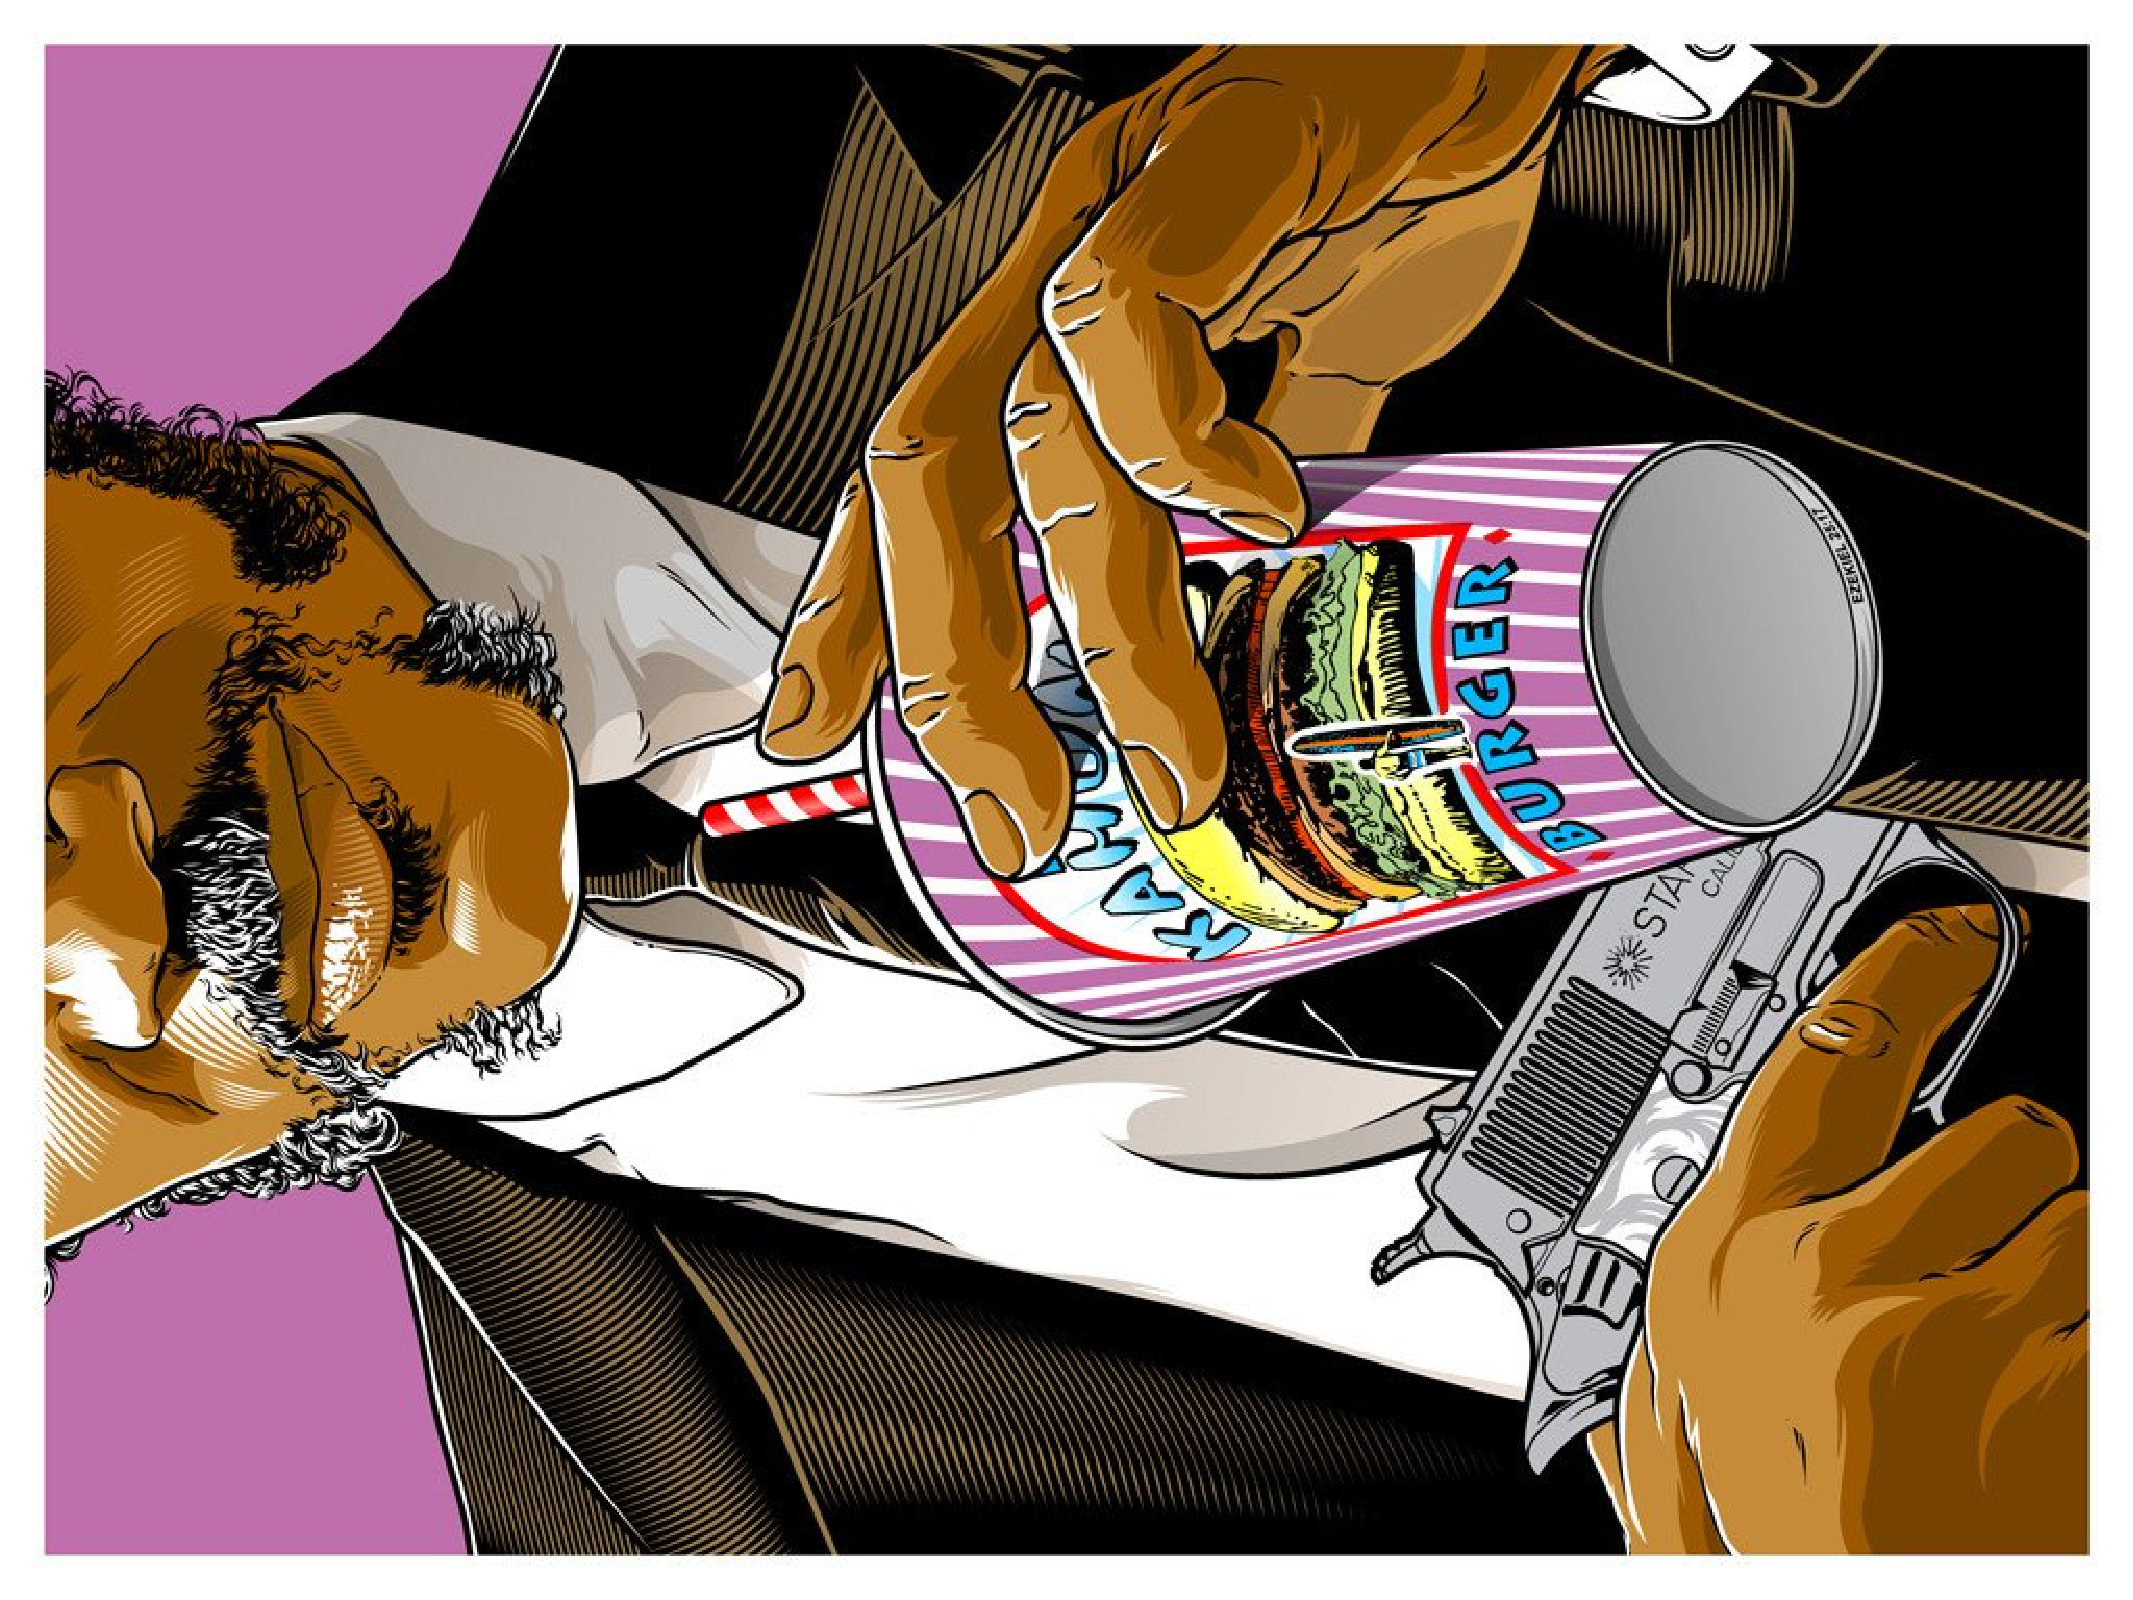
\includegraphics[height=5cm, width=6cm, angle=270]{pop1.pdf}
\end{minipage}
\hfill
\begin{minipage}[h!]{0.3\linewidth}
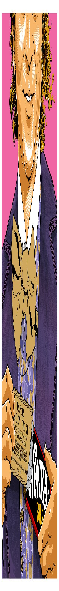
\includegraphics[height=6cm, width=5cm]{pop7.pdf}
\end{minipage}
\hfill
\begin{minipage}[h!]{0.3\linewidth}
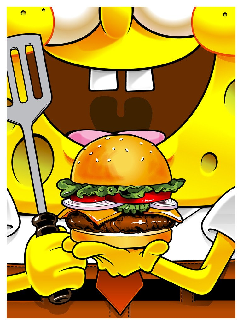
\includegraphics[height=6cm, width=5cm]{pop8.pdf}
\end{minipage}
\hfill
\begin{minipage}[h!]{0.3\linewidth}
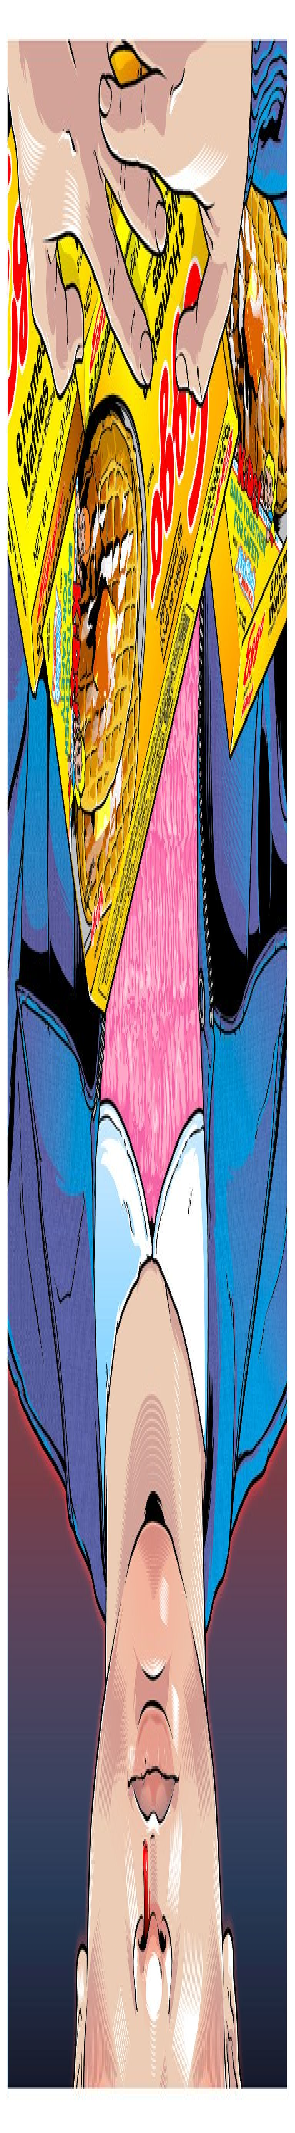
\includegraphics[height=6cm, width=5cm, angle=180]{pop2.pdf}
\end{minipage}
\hfill
\begin{minipage}[h!]{0.3\linewidth}
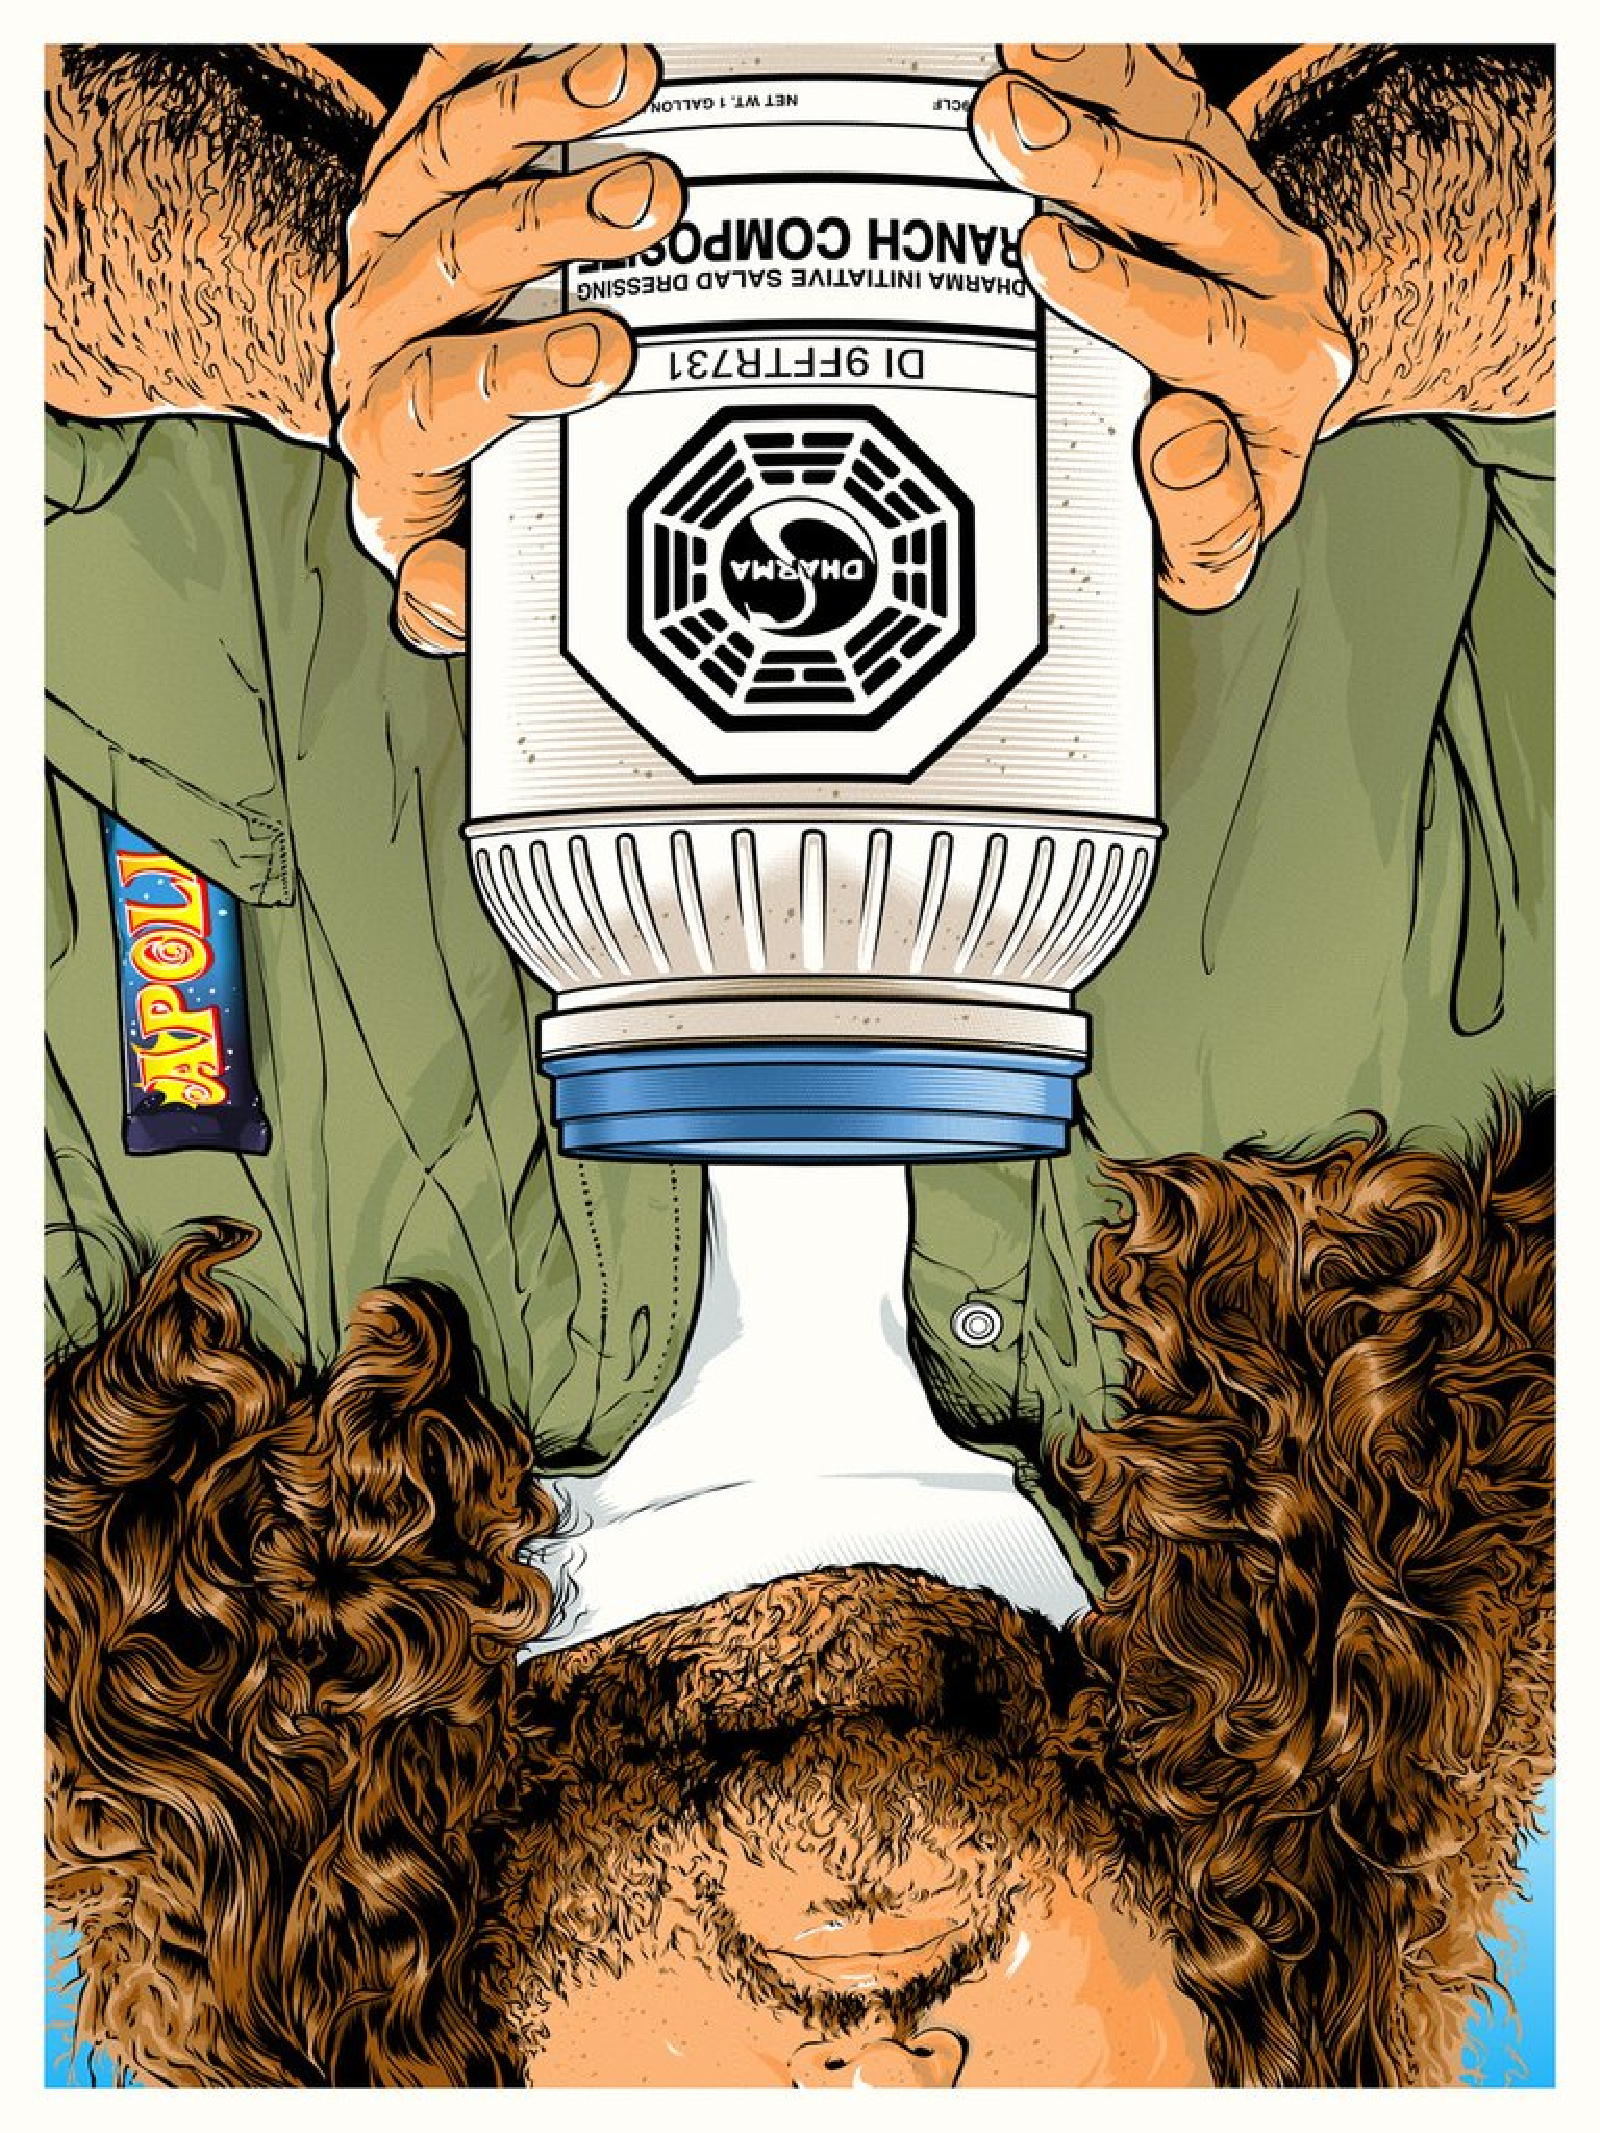
\includegraphics[height=6cm, width=5cm, angle=180]{pop10.pdf}
\end{minipage}
\hfill
\begin{minipage}[h!]{0.3\linewidth}
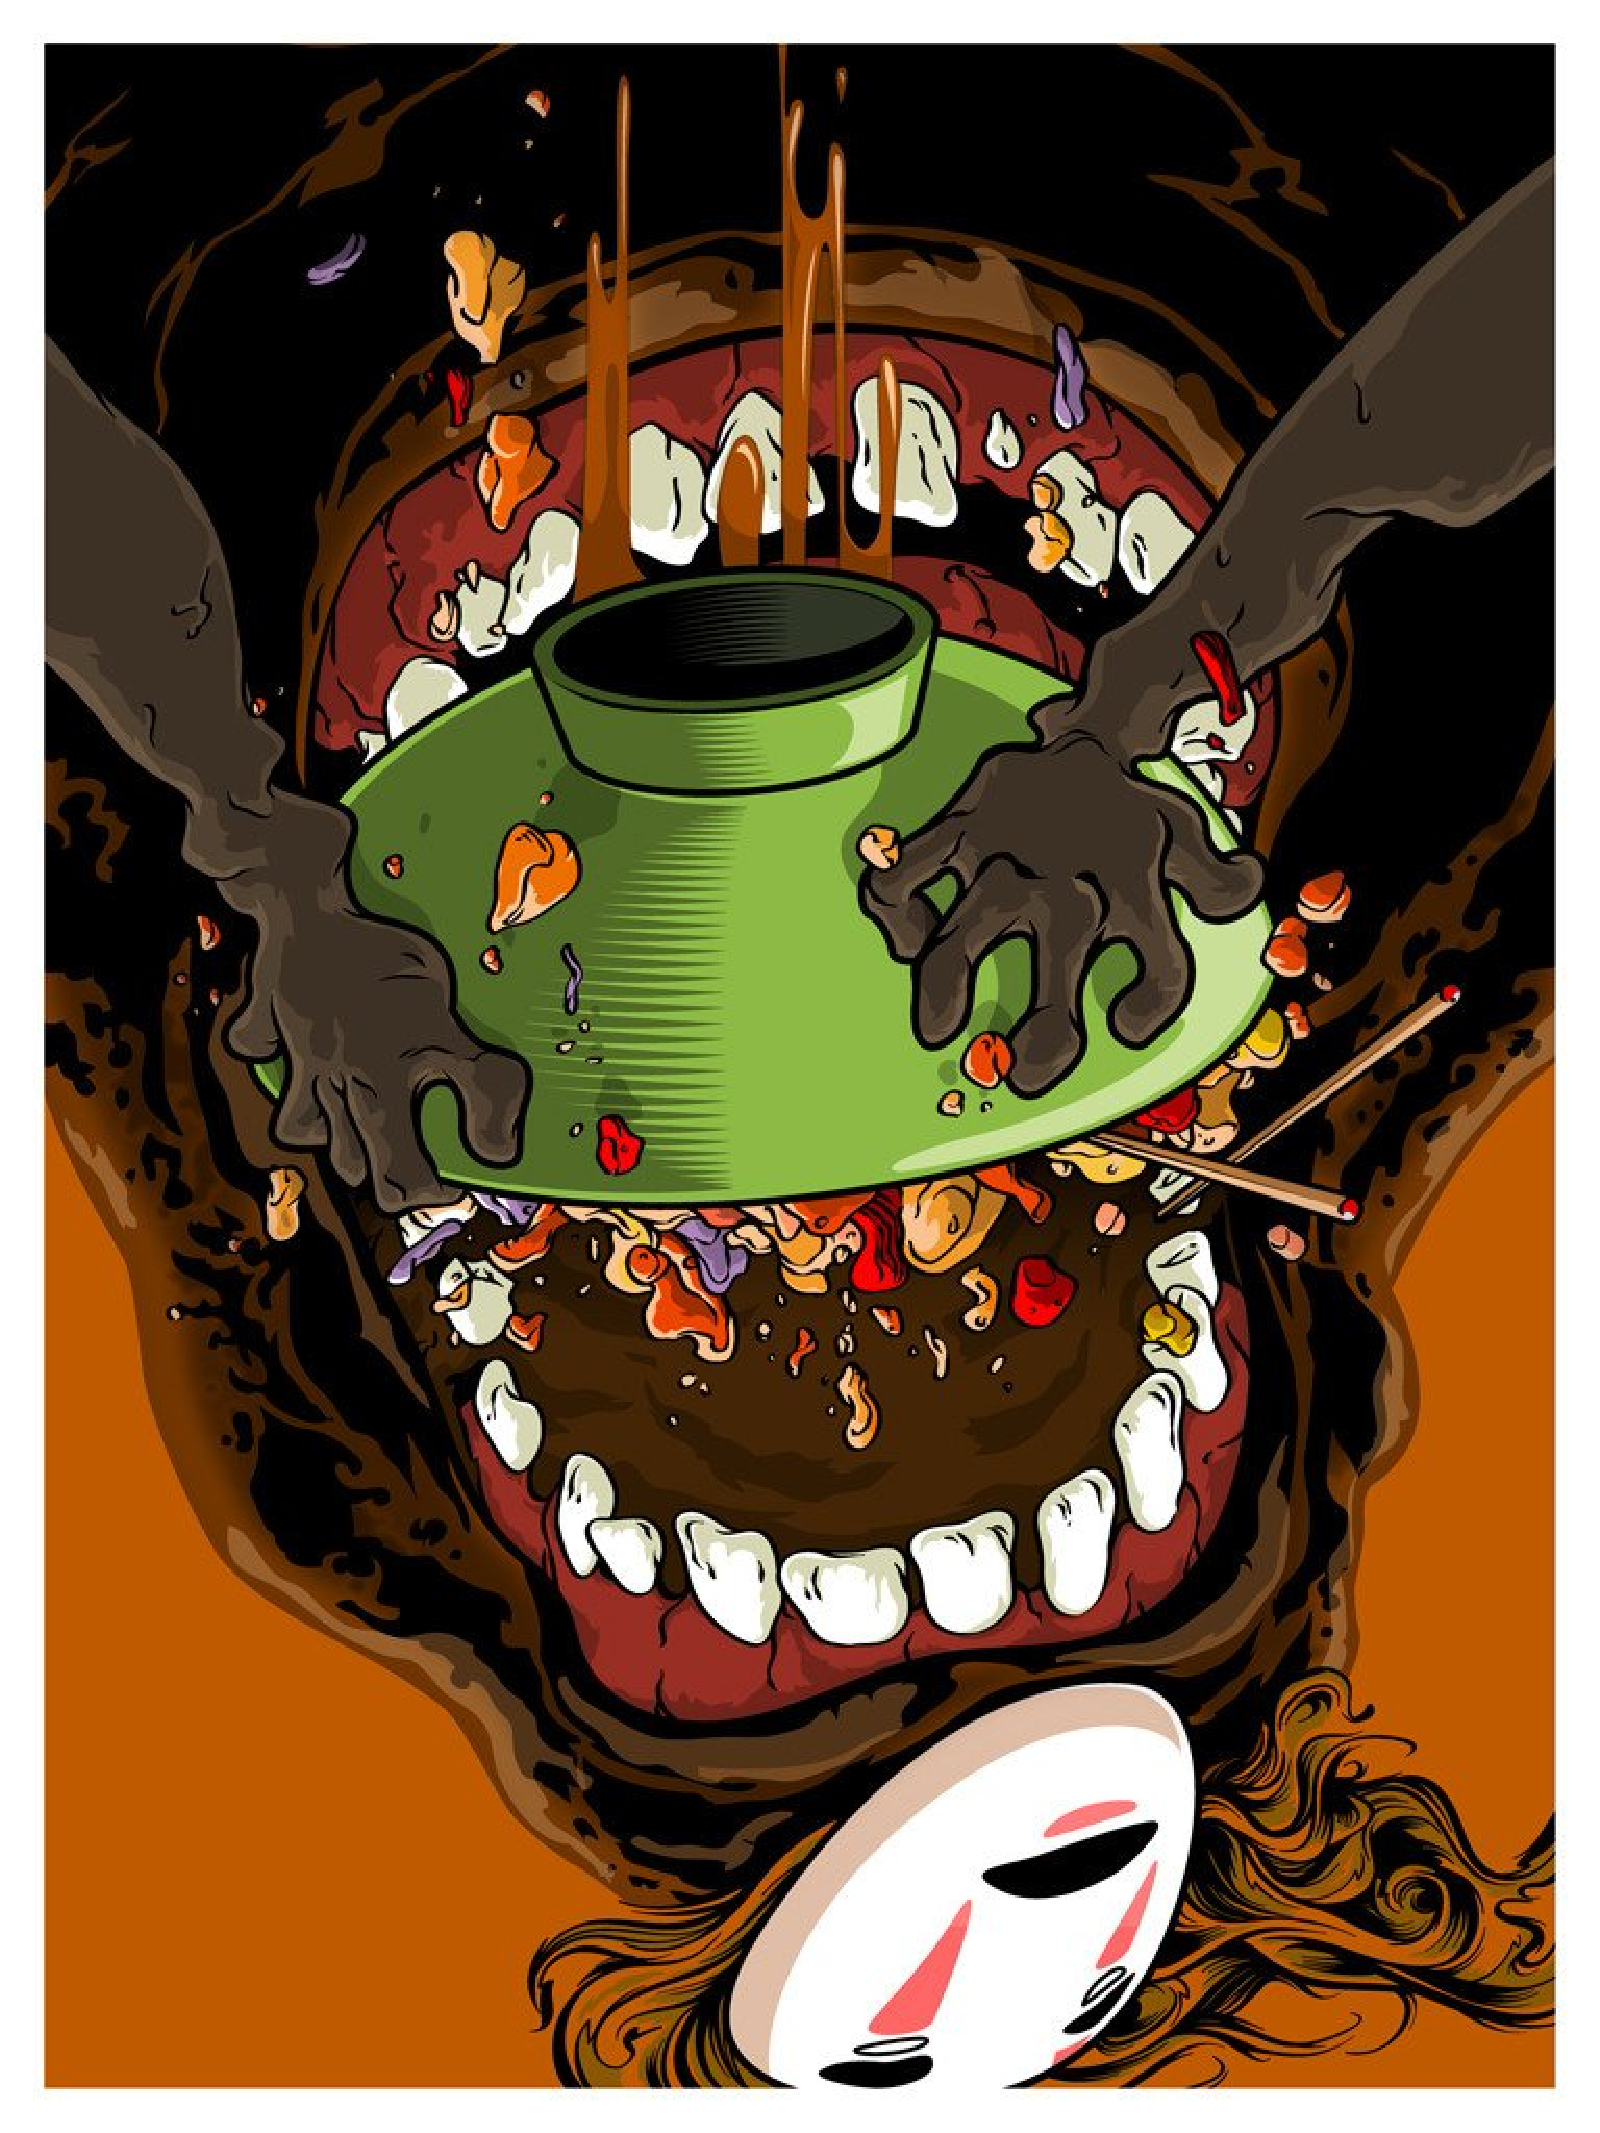
\includegraphics[height=6cm, width=5cm, angle=180]{pop6.pdf}
\end{minipage}
\caption{Поп-арт}
\label{fig:1figs}

\end{figure}

\newpage

\section{Угроза}

{\fontspec{Phorssa}{Ты хотел меня отчислить, но делал это без уважения. Поэтому я буду звать тебя Филипп Валерьевич. Муахаха}}

\end{document}
